%!TEX root = ../../../adrien_gomar_phd.tex

To assess the capability of harmonic balance operator define 
in Eq.~\eqref{eq:sm_hb_mono_source_term_analytic} for the mono-frequential
formulation or in Eq.~\eqref{eq:sm_multi_spectral_operator} 
its multi-frequential equivalent to
capture time-periodic fields, it is tested on a pure
harmonic signal of the form
\begin{equation}
    \label{eq:sum_sin}
    u(t) = \cos(\omega t) + \sin(2 \omega t) +
    \cos(3 \omega t) + \sin(4 \omega t) + \cos(5 \omega t),
\end{equation}
where $\omega = 2 \pi f$ and $f$ is the temporal frequency of
the phenomenon.
The analytical time-derivative is then:
\begin{equation}
    \label{eq:sum_sin_deriv}
    \frac{\partial u}{\partial t} = 
    \omega\left[ -\sin(\omega t) + 
    2\cos(2 \omega t) -
    3\sin(3 \omega t) + 
    4\cos(4 \omega t) -
    5\sin(5 \omega t)\right]
\end{equation}
This derivative will be compared to the estimation
given by the HB operator defined in Eq.~\eqref{eq:sm_hb_mono_source_term_analytic}
or Eq.~\eqref{eq:sm_multi_spectral_operator}, depending 
on the formulation,
and to two finite difference schemes,
a second-order centered scheme:
\begin{equation}
    \frac{\partial u}{\partial t} (t=t_q) \approx 
    \frac{u^{q+1} - u^{q-1}}{2 \Delta t},
    \label{eq:hb_op_center2}
\end{equation}
and a fourth-order centered scheme:
\begin{equation}
    \frac{\partial u}{\partial t} (t=t_q) \approx 
    \frac{-u^{q+2} + 8 u^{q+1} - 8 u^{q-1} + u^{q-2}}{12\Delta t}.
    \label{eq:hb_op_center4}
\end{equation}

The application of these three schemes applied 
to the estimation of the time-derivative of signal Eq.~\eqref{eq:sum_sin}
is shown
in Fig.~\ref{fig:hb_operator_sample}.
\begin{figure}[htbp]
  \centering
  \subfigure[$7$ samples]{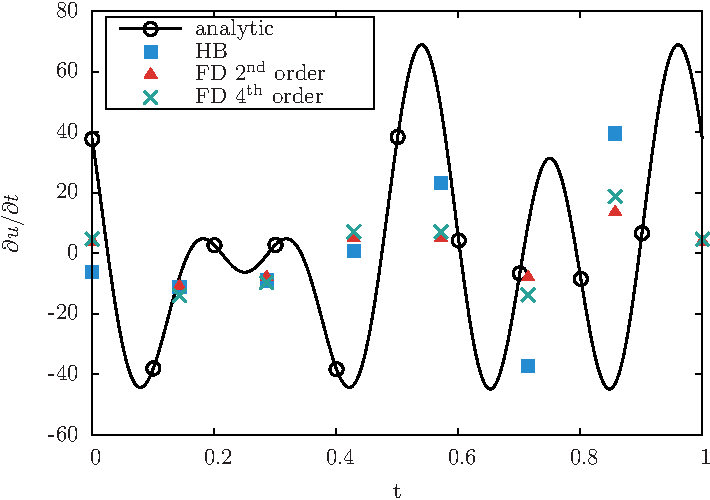
\includegraphics[width=.4\textwidth]{HB_OPERATOR_PAPER_S7.pdf}}
  \subfigure[$11$ samples]{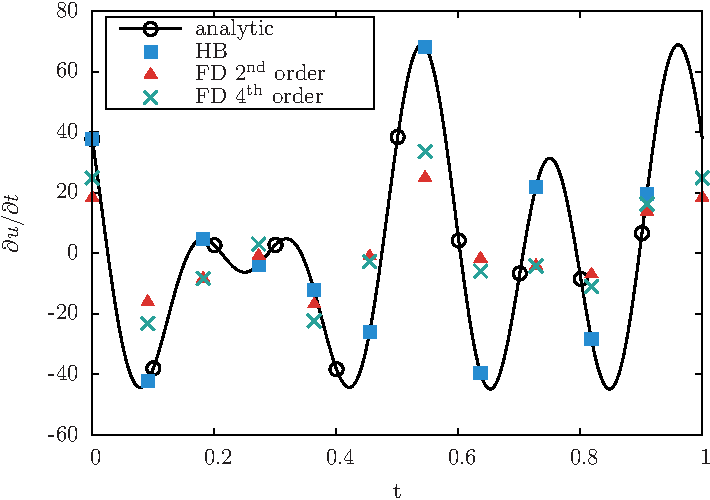
\includegraphics[width=.4\textwidth]{HB_OPERATOR_PAPER_S11.pdf}}
  \subfigure[$15$ samples]{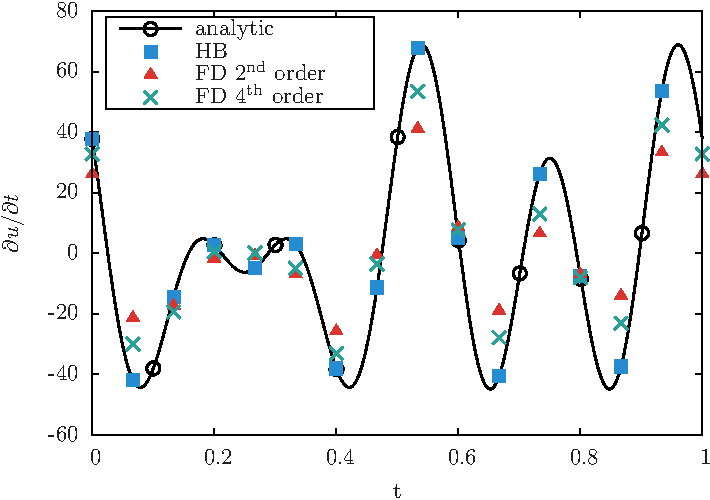
\includegraphics[width=.4\textwidth]{HB_OPERATOR_PAPER_S15.pdf}}
  \subfigure[$19$ samples]{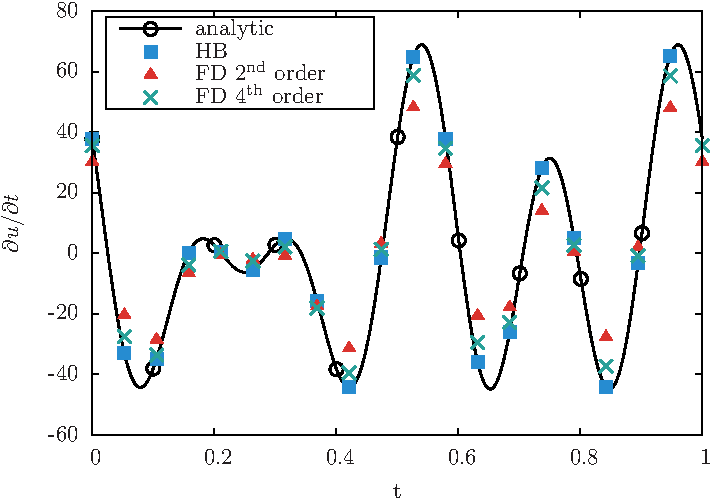
\includegraphics[width=.4\textwidth]{HB_OPERATOR_PAPER_S19.pdf}}
  \caption{Time-derivative estimation by the harmonic balance operator,
  the 2\textsuperscript{nd} order and 4\textsuperscript{th} finite difference schemes.}
  \label{fig:hb_operator_sample}
\end{figure}
Four samples
are tested: $7$, $11$, $15$ and $19$. This corresponds
to respectively $3$, $5$, $7$ and $9$ harmonics
for the HB operator. One can see that, the more the number
of samples, the better the prediction of the time-derivative.
As expected, the 4\textsuperscript{th} order finite difference
scheme does a better job than the 2\textsuperscript{nd} order.
For $19$ samples, the 4\textsuperscript{th} order finite difference
scheme almost fits the analytical solution. In opposite,
the HB operator prediction is superimpose with the analytical solution
with $11$ samples, i.e. $N=5$ harmonics. After that, increasing the
number of harmonics (or samples, recall that the number of samples
in the HB is equal to $2N+1$ with $N$ the number of harmonics)
does not improve the solution as it is already superimposed with
the analytical results.

To quantitatively analyze the results, the 
$\mathcal{L}_2$-norm of the absolute error between the analytic
derivative and the estimation given by the different schemes
is plotted in Fig.~\ref{fig:hb_operator_error}.
\begin{figure}[htb]
  \centering
   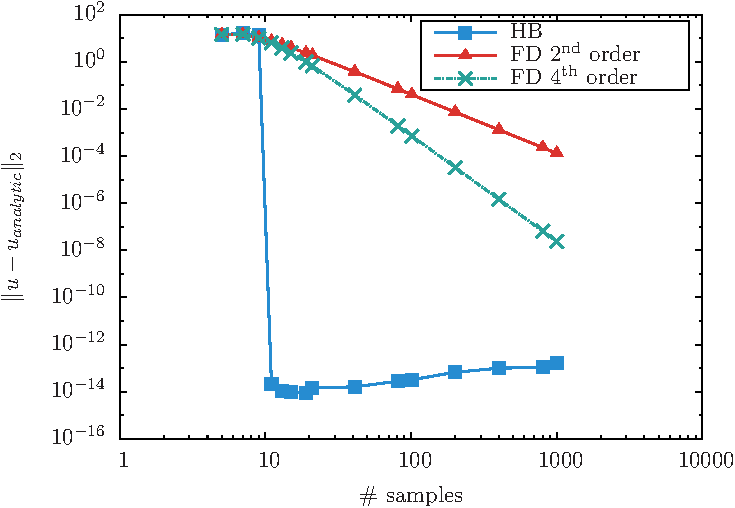
\includegraphics[width=.55\textwidth]{HB_OPERATOR_ERROR.pdf}
   \caption{$\mathcal{L}_2$-norm of the error for each time-derivative
   schemes.}
  \label{fig:hb_operator_error}
\end{figure}
One can observe the classical converging slope
equal to the order of the finite-difference schemes for the
$2$\textsuperscript{nd} and the $4$\textsuperscript{th}
order finite difference schemes. 
Adding more samples constantly improves the estimation of 
the time-derivative.
Conversely, as a spectral operator, the HB time-derivative scheme 
has a different behavior. When the Nyquist-Shannon 
criteria~\cite{Nyquist1928, Shannon1949} is not
satisfied, the error is high as Fig.~\ref{fig:hb_operator_sample}
suggest. But as soon as this criteria is satisfied, the error
drastically decreases by about $15$ order of magnitude.
Actually, on pure
harmonic signals, the HB operator is exact as soon as the time
sampling satisfies the Shannon criteria. The $\approx 10^{-13}$
remaining error is due to round-off errors.
From this study, it can be infer that the behavior
of the harmonic balance operator is not monotonic
and needs thus a deeper investigation.